\documentclass[10pt]{extarticle}
\title{}
\author{Avinash Iyer}
\date{}
\usepackage[shortlabels]{enumitem}


%paper setup
\usepackage{geometry}
\geometry{letterpaper, portrait, margin=1in}
\usepackage{fancyhdr}

%symbols
\usepackage{amsmath}
\usepackage{amssymb}
\usepackage{amsthm}
\usepackage{mathtools}
\usepackage{hyperref}
\usepackage{gensymb}
\usepackage{multirow,array}

\newtheorem*{remark}{Remark}
\usepackage[T1]{fontenc}
\usepackage[utf8]{inputenc}

%chemistry stuff
%\usepackage[version=4]{mhchem}
%\usepackage{chemfig}

%plotting
\usepackage{pgfplots}
\usepackage{tikz}
\tikzset{middleweight/.style={pos = 0.5, fill=white}}
\tikzset{weight/.style={pos = 0.5, fill = white}}
\tikzset{lateweight/.style={pos = 0.75, fill = white}}
\tikzset{earlyweight/.style={pos = 0.25, fill=white}}

%\usepackage{natbib}

%graphics stuff
\usepackage{graphicx}
\graphicspath{ {./images/} }
\usepackage[style=numeric, backend=biber]{biblatex} % Use the numeric style for Vancouver
\addbibresource{the_bibliography.bib}
%code stuff
%when using minted, make sure to add the -shell-escape flag
%you can use lstlisting if you don't want to use minted
%\usepackage{minted}
%\usemintedstyle{pastie}
%\newminted[javacode]{java}{frame=lines,framesep=2mm,linenos=true,fontsize=\footnotesize,tabsize=3,autogobble,}
%\newminted[cppcode]{cpp}{frame=lines,framesep=2mm,linenos=true,fontsize=\footnotesize,tabsize=3,autogobble,}

%\usepackage{listings}
%\usepackage{color}
%\definecolor{dkgreen}{rgb}{0,0.6,0}
%\definecolor{gray}{rgb}{0.5,0.5,0.5}
%\definecolor{mauve}{rgb}{0.58,0,0.82}
%
%\lstset{frame=tb,
%	language=Java,
%	aboveskip=3mm,
%	belowskip=3mm,
%	showstringspaces=false,
%	columns=flexible,
%	basicstyle={\small\ttfamily},
%	numbers=none,
%	numberstyle=\tiny\color{gray},
%	keywordstyle=\color{blue},
%	commentstyle=\color{dkgreen},
%	stringstyle=\color{mauve},
%	breaklines=true,
%	breakatwhitespace=true,
%	tabsize=3
%}
% text + color boxes
\usepackage[most]{tcolorbox}
\tcbuselibrary{breakable}
\newtcolorbox{problem}[1]{colback = white, title = {#1}, breakable}
\newtcolorbox{solution}{colback = white, colframe = black!75!white, title = Solution, breakable}
%including PDFs
%\usepackage{pdfpages}
\setlength{\parindent}{0pt}
\usepackage{cancel}
\pagestyle{fancy}
\fancyhf{}
\rhead{Avinash Iyer}
\lhead{Math 212: Homework 2}
\newcommand{\card}{\text{card}}
\newcommand{\ran}{\text{ran}}
\newcommand{\N}{\mathbb{N}}
\newcommand{\Q}{\mathbb{Q}}
\newcommand{\Z}{\mathbb{Z}}
\newcommand{\R}{\mathbb{R}}
\begin{document}
  \textbf{Disclaimer: Questions out of the 7th Edition of the Textbook}
  \begin{problem}{12.4}
    \begin{description}[font=\normalfont]
      \item[2:] \hfill
        \begin{center}
          \begin{tabular}{c|ccc}
            x\textbackslash y & -1 & 0 & 1 \\
            \hline
            2 & 4 & 6 & 8 \\
            3 & 1 & 3 & 5\\
            \hline
          \end{tabular}
        \end{center}
      \item[6:] The table cannot represent a linear function, as the difference between adjacent elements with constant $x$ is different in the case of $x=0$ and $x=1$.
      \item[8:] The linear function that passes through the points $(4,0,0)$, $(0,3,0)$, and $(0,0,2)$ is
        \[
          3x + 4y + 6z = 12
        \] 
      \item[12:] \hfill
        \begin{enumerate}[(a)]
          \item $5x - 3y - 13 = z$
          \item The contour diagram is below:
            \begin{center}
              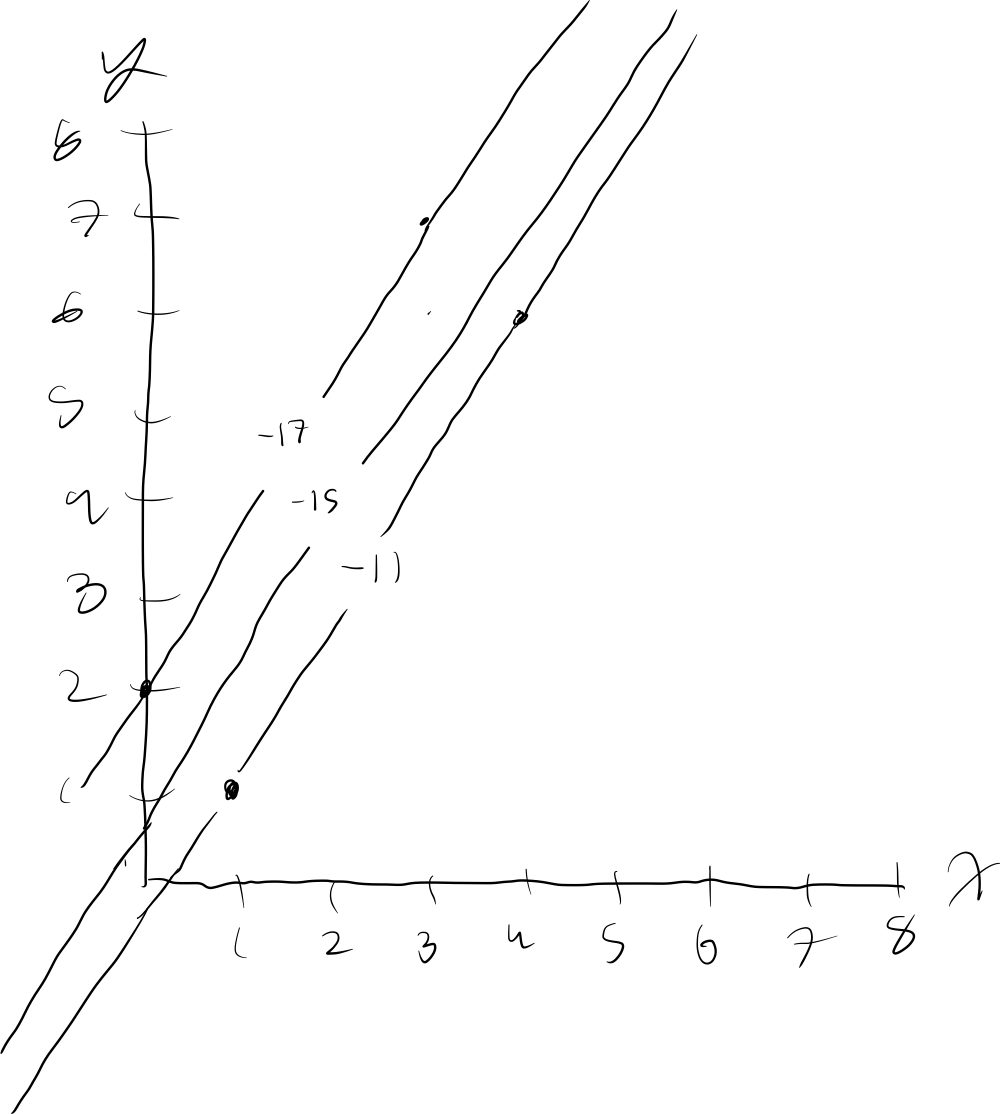
\includegraphics[width=10cm]{images/12_4_12_b.png}
            \end{center}
        \end{enumerate}
      \item[16:] \hfill
        \begin{enumerate}[(a)]
          \item $f$ is a linear function.
          \item $m$ is in dollars/month, and $t$ is in dollars/gigabyte.
          \item $f(3,8) = 269$, meaning that it costs \$269 in total to use 8 gigabytes of data over 3 months.
        \end{enumerate}
      \item[22:]\hfill
        \[
          z = 2x - y + 4
        \] 
      \item[52:] The contours of $f(x,y) = 3x + 2y$ are of the form $c = 3x + 2y$, meaning they have slope $-\frac{3}{2}$
    \end{description}
  \end{problem}
  \begin{problem}{12.5}
    \begin{description}[font=\normalfont]
      \item[2:]\hfill
        \begin{enumerate}[(a)]
          \item II
          \item I
        \end{enumerate}
      \item[6:]\hfill
        \[
          f(x,y,z) = (x-a)^2 + (y-b)^2 + (z-c)^2
        \] 
      \item[8:] Elliptical Paraboloid
      \item[16:]\hfill
        \begin{enumerate}[(a)]
          \item II
          \item III
          \item IV
          \item I
        \end{enumerate}
      \item[28:]\hfill
        \[
          g(x,y,z) = 2x + 3y - z
        \] 
      \item[30:]\hfill
        \begin{enumerate}[(a)]
          \item The surface is akin to all values of $z$ such that $z = \sqrt{1-x^2-y^2}$, which is only the case if $z = 1$ at $(x,y) = (0,0)$ and $x^2 + y^2 = 1$ at $z = 0$. The contours must be circles.
          \item $g(x,y,z) = x^2 + y^2 - z$, where $c = 1$.
        \end{enumerate}
    \end{description}
  \end{problem}
  \begin{problem}{12.6}
    \begin{description}[font=\normalfont]
      \item[2:] If $x=0$ and $y=2$, then $\sqrt{2x-y}$ is not defined, so the function is not continuous on $x^2 + y^2 \leq 4$.
      \item[8:] \hfill
        \[
          \lim_{(x,y) \rightarrow (0,0)} f(x,y) = 0
        \] 
      \item[10:] \hfill
        \[
          \lim_{(x,y) \rightarrow (0,0)} f(x,y) = 0
        \] 
      \item[18:] When approaching along the positive $y$ axis, we have that the limit equals $-1$, while approaching along the positive $x$ axis, we have that the limit equals $1$.
    \end{description}
  \end{problem}
  \begin{problem}{13.1:}
    \begin{description}[font=\normalfont]
      \item[2:]\hfill
        \begin{itemize}
          \item $\vec{a} = \langle 2,1\rangle$
          \item $\vec{b} = \langle 2,0\rangle$
          \item $\vec{c} = \langle -2,0\rangle$
          \item $\vec{d} = \langle -2,2\rangle$
          \item $\vec e = \langle -2,-1\rangle$
        \end{itemize}
      \item[4:]\hfill \[\vec v = \langle 3,4 \rangle\]
      \item[8:] \hfill \[\vec v = -5\hat{i} - 4\hat{j}\]
      \item[12:]\hfill \[\vec v = -6\hat{i} -5\hat{j} + 11\hat{k}\]
      \item[16:] \hfill \[\Vert \vec z \Vert = \sqrt{11}\]
      \item[36:] \hfill
        \begin{align*}
          \vec u &= \langle 3.2,3.2\rangle\\
          \vec v &= \langle -3.2,-3.2\rangle
        \end{align*}
      \item[40:] Counterclockwise from $\vec v$, they are $\vec v - \vec u$, $-\vec u$, $-\vec v$, and $\vec v - \vec u$.
      \item[46:]\hfill
        \begin{enumerate}[(i)]
          \item $\Vert \vec{OB} \Vert = \sqrt{1+3} = 2$
          \item $\Vert \vec{OC}\Vert = \sqrt{1 + 1/3 + 8/3} = 2$
          \item $\Vert \vec{CB}\Vert = \sqrt{8/3 + 4/3} = 2$
          \item $\Vert \vec{AB}\Vert = \sqrt{(2-1)^2 + 3} = 2$
        \end{enumerate}
    \end{description}
  \end{problem}
\end{document}
